\documentclass[oneside,a4paper,12pt]{article}
\usepackage[english,brazilian]{babel}
\usepackage[alf]{abntex2cite}
\usepackage[utf8]{inputenc}
\usepackage[T1]{fontenc}
\usepackage[top=15mm, bottom=15mm, left=15mm, right=15mm]{geometry} %Para alterações no margens da folha.
\usepackage{framed}
\usepackage{booktabs}
\usepackage{color}
\usepackage{hyperref}
\usepackage{graphicx}
\usepackage{float}
\graphicspath{{./Figuras/}}    
\definecolor{shadecolor}{rgb}{0.8,0.8,0.8}

\usepackage[none]{hyphenat} %Evita a hifenização no documento

\usepackage{multicol}
\columnsep=10mm %Espaçamento entre colunas.

\newcommand{\ESCOLA}{EREM Regina Pacis}
\newcommand{\SERIE}{\textbf{3 EMSI A}}
\newcommand{\PROFESSOR}{Prof. Leandro Vieira}
\newcommand{\DATA}{\textbf{abril de 2020}}
\newcommand{\CONTEUDO}{\LARGE \textbf{Atividade de Geometria}}
\newcommand{\FRASE}{\flushright{"Sem liberdade de criticar, não existe elogio sincero."\\\textbf{Pierre Beaumarchais}}}

\begin{document}
\pagestyle{empty}
\DATA

\begin{center}		 	
\ESCOLA \\
\SERIE \\
\PROFESSOR \\
\CONTEUDO
\end{center}

\begin{enumerate}
\item 
	\begin{enumerate}
	\item item
	\item item
	\item item
	\item item
	\item item
	\end{enumerate}
	
\item Questão Figura \ref{rotulodafigura}:

	\begin{figure}[h]
	\center
	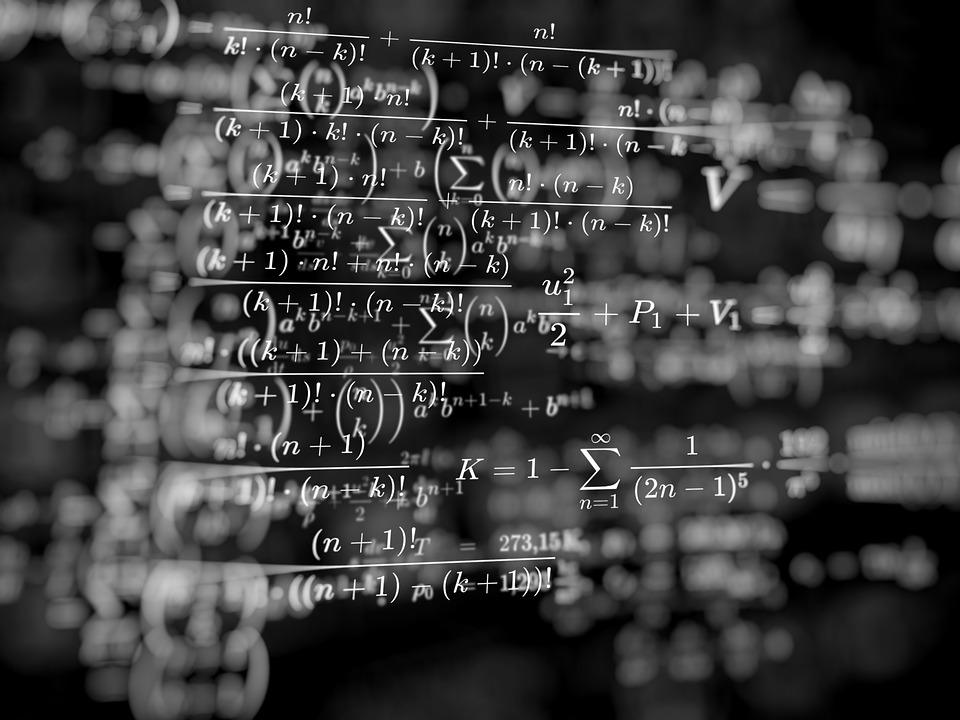
\includegraphics[width=8cm]{Figuras/imagem.jpg}
	\caption{Legenda da Figura}
	\label{rotulodafigura}
	\end{figure}

	\begin{enumerate}
	\item item
	\item item
	\item item
	\item item
	\item item
	\end{enumerate}
	
\end{enumerate}

\FRASE
\end{document}